
    \documentclass{article}
    \usepackage{graphicx}
    \usepackage{booktabs}
    \usepackage{float}
    \title{QKD Network Analysis Report}
    \date{2025-02-17}
    \begin{document}
    \maketitle

    \section{Network Characteristics}
    Number of nodes: 10 \\
    Number of edges: 39 \\
    Average degree: 7.80 \\
    Average clustering coefficient: 0.907 \\
    Average shortest path length: 1.13

    \section{QKD Performance}
    Average key rate: 6.48e+02 bits/s \\
    Average QBER: 0.054 \\
    Maximum link distance: 12.1 km

    \section{Link Prediction Performance}
    \begin{table}[H]
    \centering
    \begin{tabular}{lcc}
    \toprule
    Metric & Mean & Std. Dev. \\
    \midrule
    AUC & 0.690 &
        0.073 \\
    AP & 0.703 &
        0.078 \\
    \bottomrule
    \end{tabular}
    \caption{Link Prediction Performance Metrics}
    \end{table}

    \section{Network Reliability}
    Edge connectivity: 5 \\
    Node connectivity: 5 \\
    Algebraic connectivity: 4.738

    \section{Figures}
    \begin{figure}[H]
    \centering
    \includegraphics[width=0.8\textwidth]{network_topology.png}
    \caption{QKD Network Topology}
    \end{figure}

    \begin{figure}[H]
    \centering
    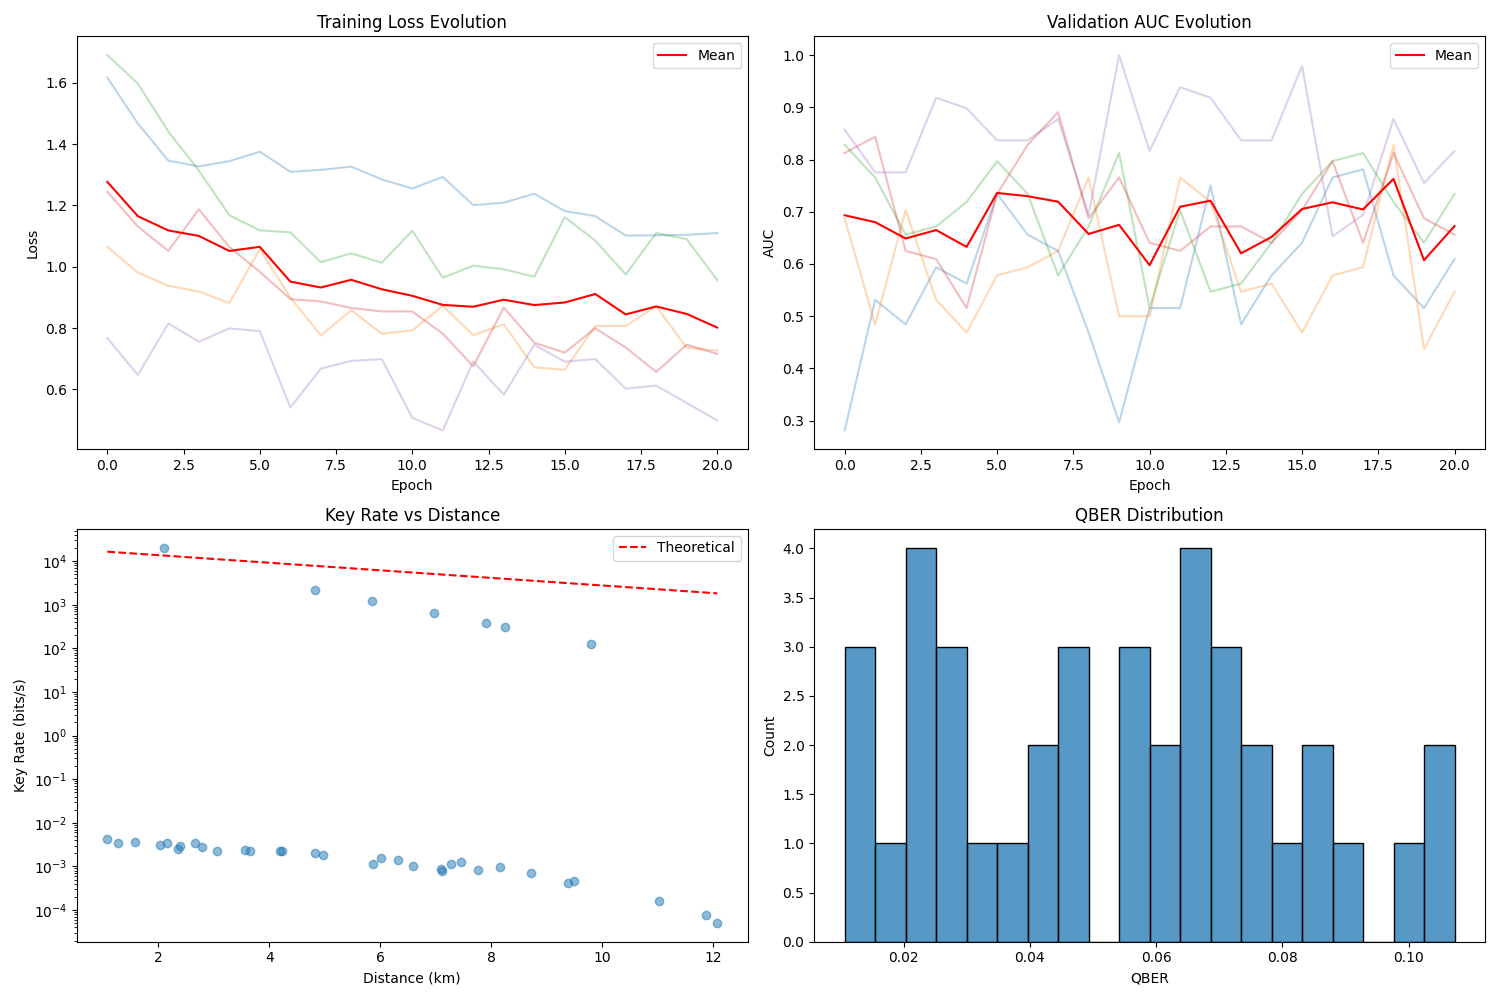
\includegraphics[width=0.8\textwidth]{training_metrics.png}
    \caption{Training and Validation Metrics}
    \end{figure}

    \begin{figure}[H]
    \centering
    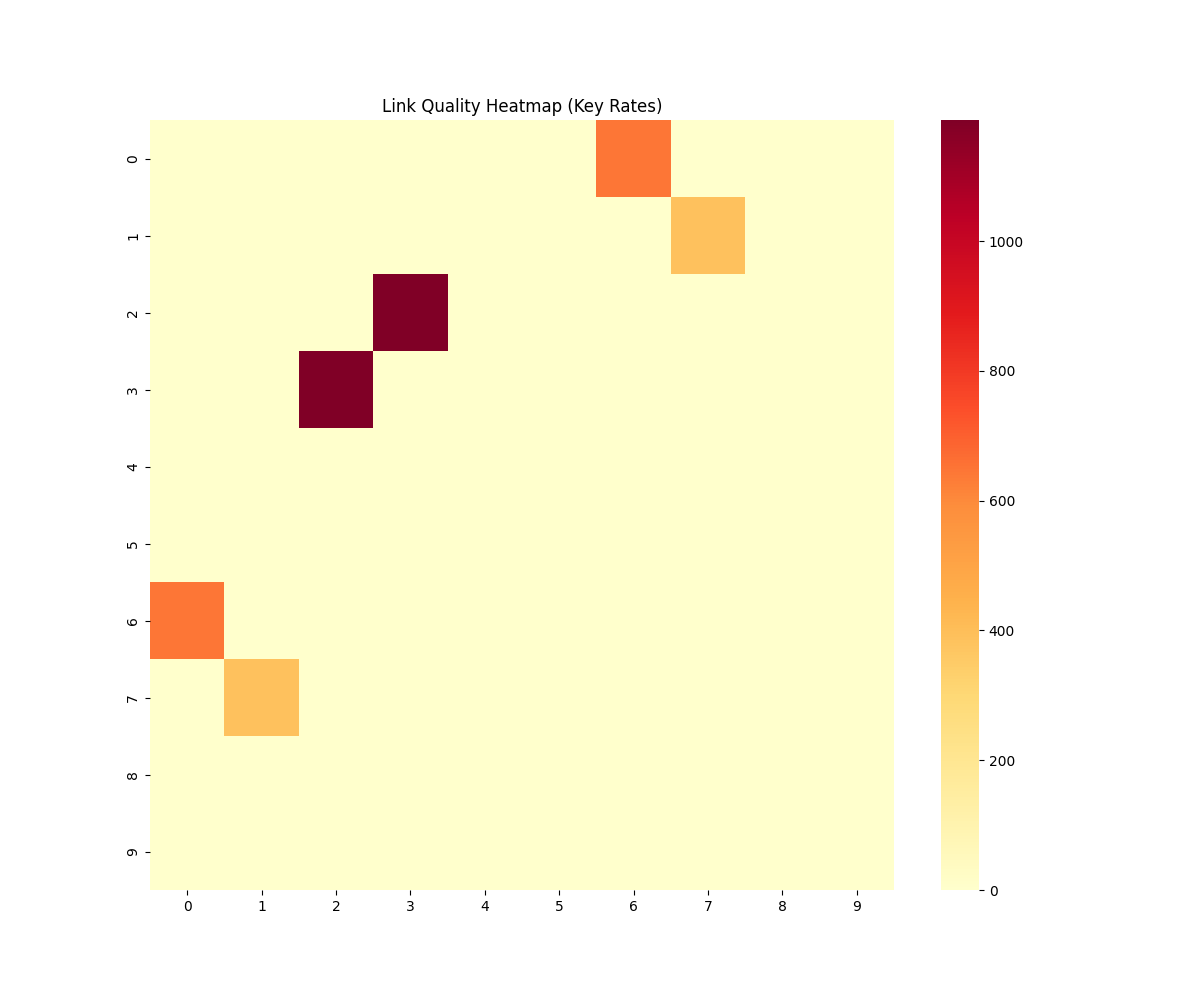
\includegraphics[width=0.8\textwidth]{link_quality_heatmap.png}
    \caption{Link Quality Heatmap}
    \end{figure}

    \end{document}
    